Since the networks are already characterized and with enough knowledge to
define which networks the phenomenon studied  is mostly likely to occur
theoretically, the following are the results of the first part of the
practical experimentation.

Iperf revealed that indeed, overloading a network average RTT time in direct
proportion to the load in-fly (relation with more data to negotiate, more
information over the network, higher RTTs), with which to demand it even more,
like including other connections can reach to the collapse making even to load
a basic website will become a task that takes a couple of minutes.

The following graphs show results in three networks characterized in ascending
seriousness of the problem. Each figure is the result of three iterations
performed in each network, without load and the two iterations performed with
extra load.

\begin{figure}[ht]
\centering
	%\rule{5.5cm}{7.1cm}
    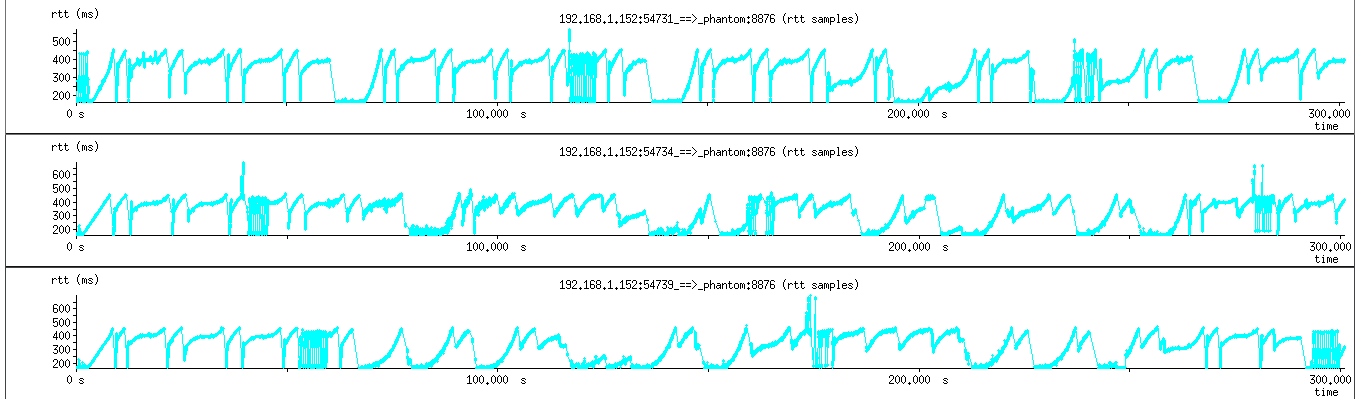
\includegraphics[width=\textwidth]{img/n_iperf_good}
\caption[Iperf: RTT graphs for a fiber network]{RTT graphs for the three test in a fiber network}
\label{fig:iperfgood}
\end{figure}%

Figure \ref{fig:iperfgood} shows the behavior of the network which, although it
has a bandwidth in the mid-high average range, but with its transmission rate
higher because it is a fiber optic network (\emph{casa\_w}). It can be
appreciated that in a state where only one application uses the entire
bandwidth, there is an increased RTT time, but not significant. In fact the
only difference compared to the following two graphs sharing network resources
applications is that there are some higher peaks, but these are not constant.
Nor is there a greater retransmission (denoted by the thinner lines). So, with
at least two data sources generating traffic, there is no significant increase
in RTT time and should not imply that the increase in the loading time for a
browsing client, or some type of problem seen in real time applications.

\begin{figure}[ht]
\centering
	%\rule{5.5cm}{7.1cm}
    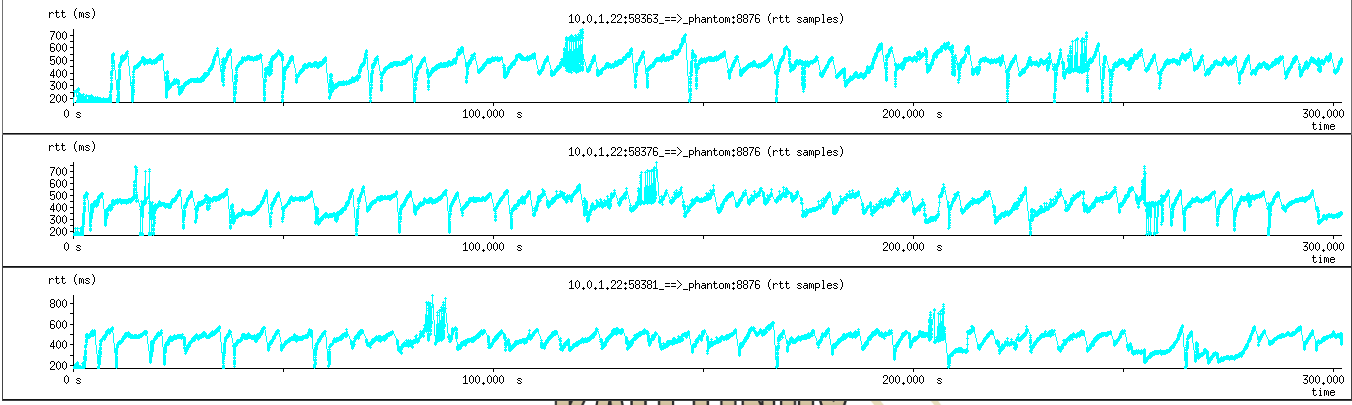
\includegraphics[width=\textwidth]{img/n_iperf_mid}
\caption[Iperf: RTT graphs for a network with minor issues]{RTT graphs for the three tests in a network with minor issues}
\label{fig:iperfmid}
\end{figure}%


For Figure \ref{fig:iperfmid}, at the beginning of the fist test (first $\sim10$ seconds) the RTT times are really small, but according to previous cases, is about the time it takes to saturate the buffers. This behavior proves that is what is occurring, specially that after this period of time RTT rise almost doubling, presenting ranges between 400 and 700 ms, but with valleys that are round to  300 ms or less. For the second and third graph in this network, the valleys are reduced and with higher values, especially in periods when the second application is making use of the resource (between about 50 and 250 seconds), being noticed particularly few times in the third chart which also shows an increase in the maximum upper 800 ms. This network corresponds to \emph{polmos\_w}.

\begin{figure}[ht]
\centering
	%\rule{5.5cm}{7.1cm}
    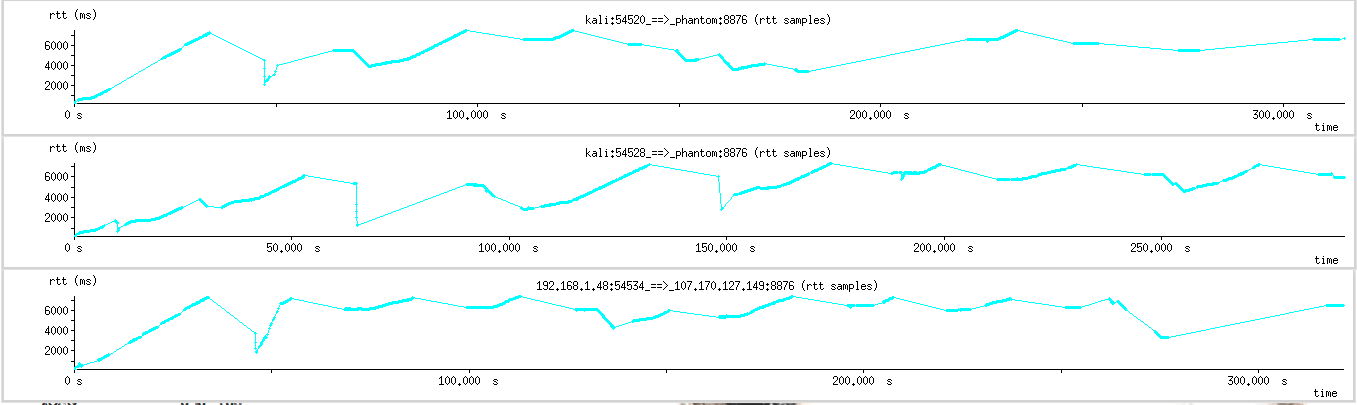
\includegraphics[width=\textwidth]{img/n_iperf_bad}
\caption[Iperf: RTT graphs for a network with bad performance]{RTT graphs for the three tests in a network with bad performance}
\label{fig:iperfbad}
\end{figure}%

In Figure \ref{fig:iperfbad} the things got to the extreme. Even for the base
case, where the times should be low, for this scenario the peaks are around 6
seconds, with a always upward trend. Also it is a constant presence of long
periods where no samples are among the packets in transit which are not
retransmitted packets (thinner lines). Current websites delayed an average of 2
seconds to load the full site, finding in the range between 1 and 7 seconds,
for the full negotiation; but here, only one package is taken almost the
same that takes a full site to load.

At first glance it seems that the case two is better than the base case, but
it can be noticed that the relay times (may be caused by loss), are up most of time,
perhaps they produced a massive drop of packets (approximately the second 70),
so having a valley at a point less than in the base case. The third graph
shows no far difference with what already found only proving the fact that
there are some serious problems in the network that makes RTTs times increase
to three or four times the normal behavior. With this times, it is almost
impossible to maintain a steady stream of data with one application, so the
use of real-time applications such as online games or web conference while web
surfing would be almost impossible, and must sacrifice any.

\begin{figure}[ht]
\centering
	%\rule{5.5cm}{7.1cm}
    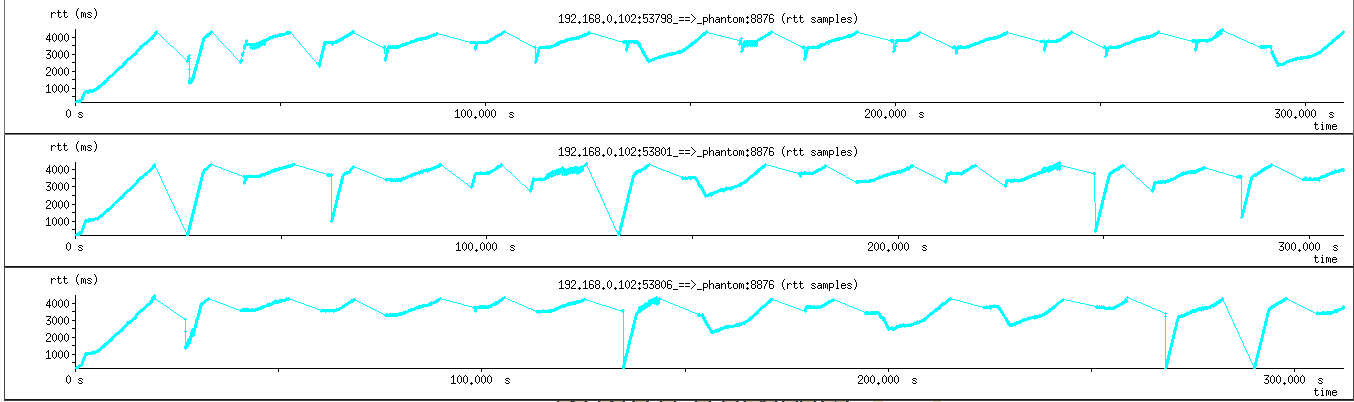
\includegraphics[width=\textwidth]{img/n_iperf_4low}
\caption[Iperf: RTT graphs for a network with DNS issues]{RTT graphs for the three tests in a network with DNS issues}
\label{fig:iperf4low}
\end{figure}%

It is interesting that for the network \emph{4low}, which presents problems with DNS resolution time was needed more than twice tries in order to perform this tests, as the website used to saturate as a second stream of data could not be loaded throwing error connection time (timeout). After the website completes its full load, having to load it before start iperf for the two cases, it could continue with the normal course of the test.
